Лескин К.А.

гр. 9892

\section*{Задание}

Установить при помощи алгоритма Маркова, обладает ли данная схема кодирования свойством взаимной однозначности. Если обладает – обосновать при помощи построенного графа, если не обладает – предъявить неоднозначно декодируемое слово и раскодировать его в алфавите сообщений двумя способами. 
\\

\textbf{Вар. 4}

\begin{tabular}{|c|c|c|c|c|c|}
    \hline
    $ a_1 $ & $ a_2 $ & $ a_3 $ & $ a_4 $ & $ a_5 $ & $ a_6 $\\
    \hline
    $ b_1b_2 $ & 
    $ b_1b_2b_2 $ & 
    $ b_2b_1b_1 $ & 
    $ b_3b_2b_1b_1 $ & 
    $ b_2b_1b_2b_3b_2b_1 $ & 
    $ b_1b_1b_2b_3b_2b_1 $\\
    \hline
\end{tabular}

\ 
\\

Обозначим элементарные коды $ \beta_{1-6} $ :

$ \beta_1 = b_1b_2 $,
$ \beta_2 = b_1b_2b_2 $,
$ \beta_3 = b_2b_1b_1 $,
$ \beta_4 = b_3b_2b_1b_1 $,
$ \beta_5 = b_2b_1b_2b_3b_2b_1 $,
$ \beta_6 = b_1b_1b_2b_3b_2b_1 $.

Учитывая, что начало $ \beta' $ не должно заканчиваться на какой-либо элементарный код, а конец $ \beta'' $ --- начинаться на него,
выпишем все нетривиальные разложения элементарных кодов $ \beta_{1-6} $:\\

$ 
\beta_1 = 
(b_1)_{\beta'}(b_2)_{\beta''} 
$
\\

$ 
\beta_2 = 
(b_1)_{\beta'}(b_2b_2)_{\beta''} = (\Lambda)_{\beta'}(b_1b_2)_{\beta_1}(b_2)_{\beta''}
$
\\

$ 
\beta_3 = 
(b_2)_{\beta'}(b_1b_1)_{\beta''} = 
(b_2b_1)_{\beta'}(b_1)_{\beta''} 
$
\\
 
$ 
\beta_4 = 
(b_3)_{\beta'}(b_2b_1b_1)_{\beta_3}(\Lambda)_{\beta''} = 
(b_3b_2)_{\beta'}(b_1b_1)_{\beta''} = 
(b_3b_2b_1)_{\beta'}(b_1)_{\beta''}
$
\\

$ % b_2b_1b_2b_3b_2b_1 
\beta_5 = 
(b_2)_{\beta'}(b_1b_2)_{\beta_1}(b_3b_2b_1)_{\beta''} =
(b_2b_1)_{\beta'}(b_2b_3b_2b_1)_{\beta''}  =
(b_2b_1b_2b_3)_{\beta'}(b_2b_1)_{\beta''}  =
(b_2b_1b_2b_3b_2)_{\beta'}(b_1)_{\beta''}
$
\\

$ 
\beta_6 = 
(b_1)_{\beta'}(b_1b_2)_{\beta_1}(b_3b_2b_1)_{\beta''} = 
(b_1b_1)_{\beta'}(b_2b_3b_2b_1)_{\beta''}  =
(b_1b_1b_2b_3)_{\beta'}(b_2b_1)_{\beta''}  =
(b_1b_1b_2b_3b_2)_{\beta'}(b_1)_{\beta''} 
$
\\

Составим множество $ M_{\beta'} $ всех начал разложений (без повторений):\\

$ 
M_{\beta'} = \{
b_1, 
b_2, 
b_2b_1, 
b_3,
b_3b_2, 
b_3b_2b_1, 
b_2b_1b_2b_3,
b_2b_1b_2b_3b_2, 
b_1b_1, 
b_1b_1b_2b_3, 
b_1b_1b_2b_3b_2
\}
$
\\

Составим множество $ M_{\beta''} $ всех концов разложений (без повторений):\\

$ 
M_{\beta''} = \{
b_2,
b_2b_2,
b_1b_1,
b_1,
b_3b_2b_1,
b_2b_3b_2b_1,
b_2b_1
\}
$
\\

Найдём $ M = (M_{\beta'} \cap M_{\beta''}) \cup \{\Lambda\} $:\\

$ M = \{
\Lambda,
b_1,
b_2,
b_2b_1,
b_3b_2b_1,
b_1b_1
\} 
$
\\

Пстроим граф с вершинами из $ M $:

\begin{figure}[hpt!]
    \centering
    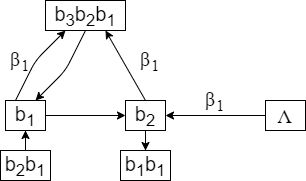
\includegraphics{photo/graph}
\end{figure}

Поскольку построенный граф не содержит ни одного цикла, проходящего через вершину, соответствующую пустому слову, \textbf{кодирование \underline{является однозначным}}.